\documentclass[11pt]{scrartcl}
\title{SampleTemplate_Assignment} %Compiled by Nuwan Bandara, ENTC, University of Moratuwa, Sri Lanka
\nonstopmode
%\usepackage[utf-8]{inputenc}
\usepackage{graphicx} % Required for including pictures
\usepackage[figurename=Figure]{caption}
\usepackage{float}    % For tables and other floats
\usepackage{verbatim} % For comments and other
\usepackage{amsmath}  % For math
\usepackage{amssymb}  % For more math
\usepackage{fullpage} % Set margins and place page numbers at bottom center
\usepackage{subcaption}
\usepackage{paralist} % paragraph spacing
\usepackage{listings} % For source code
\usepackage{subfig}   % For subfigures
%\usepackage{physics}  % for simplified dv, and 
\usepackage{enumitem} % useful for itemization
\usepackage{siunitx}  % standardization of si units
\usepackage{hyperref}
\usepackage{tikz,bm} % Useful for drawing plots
\usepackage{circuitikz}
\bibliographystyle{IEEEtran}
\usepackage{cite}

%%% Colours used in field vectors and propagation direction
\definecolor{mycolor}{rgb}{1,0.2,0.3}
\definecolor{brightgreen}{rgb}{0.4, 1.0, 0.0}
\definecolor{britishracinggreen}{rgb}{0.0, 0.26, 0.15}
\definecolor{cadmiumgreen}{rgb}{0.0, 0.42, 0.24}
\definecolor{ceruleanblue}{rgb}{0.16, 0.32, 0.75}
\definecolor{darkelectricblue}{rgb}{0.33, 0.41, 0.47}
\definecolor{darkpowderblue}{rgb}{0.0, 0.2, 0.6}
\definecolor{darktangerine}{rgb}{1.0, 0.66, 0.07}
\definecolor{emerald}{rgb}{0.31, 0.78, 0.47}
\definecolor{palatinatepurple}{rgb}{0.41, 0.16, 0.38}
\definecolor{pastelviolet}{rgb}{0.8, 0.6, 0.79}

\begin{document}
\begin{center}
	\hrule
	\vspace{.4cm}
	{\textbf { \large [ENXXXX] --- [Module Descriptive Name]}}
\end{center}
{\textbf{Student Name:}\ [ABC DEFGH] \hspace{\fill} \textbf{Submitted Date:} [April 02, 2021]   \\
{ \textbf{Student Number:}} \ [123456X] \hspace{\fill} \textbf{Assignment Number:} [1] \\
	\hrule

\bigskip

\textit{The necessary changes to be executed, in order to transform this template to your assignment could be found within square brackets - [ ] or with the initiation of the word "Sample". The compact style of documentation is ideal to follow in an assignment where the page limit is defined and critical}.

Sample Text: Entire code flow for the assignment is accessible via, \\ 
\textbf{\url{[The Open-source link for the assignment if any]}}

\paragraph*{Problem 1} %\hfill \newline
Sample Question: A part of the code for a linear classifier for CIFAR10 given in listing 1. For our linear classifier, the score function is $f(x) = Wx + b$, and the loss function is the mean sum of squared errors function.
\newline
Sample Answer: Lorem Ipsum is simply dummy text of the printing and typesetting industry. Lorem Ipsum has been the industry's standard dummy text ever since the 1500s, when an unknown printer took a galley of type and scrambled it to make a type specimen book. It has survived not only five centuries, but also the leap into electronic typesetting, remaining essentially unchanged. It was popularised in the 1960s with the release of Letraset sheets containing Lorem Ipsum passages, and more recently with desktop publishing software like Aldus PageMaker including versions of Lorem Ipsum.\cite{A1} (The citations could be added using cite package).

\begin{enumerate}[label=(\alph*)]
\item Sample Sub-question: Implement gradient descent and run for 300 epochs.
\newline Sample Answer: Lorem Ipsum is simply dummy text of the printing and typesetting industry. Lorem Ipsum has been the industry's standard dummy text ever since the 1500s, when an unknown printer took a galley of type and scrambled it to make a type specimen book. It has survived not only five centuries, but also the leap into electronic typesetting, remaining essentially unchanged.

\begin{itemize}[noitemsep,nolistsep]
%\itemsep-1em
    \item \textit{Item 1} 
    \item \textit{Item 2} 
    \item \textit{Item 3} 
    \item \textit{Item 4} 
    \vspace{-0.2cm}
\end{itemize}

\textit{The mathematical equations could be included using math package as indicated here.} 
\begin{equation}
    f(x_i,W,b) = Wx_i + b
\end{equation}
\textit{Mathematical expressions could be added within the text passage as follows. Sample Text: Here, $x_i \in R^D$ each associated with a label $y_i$. Here $i=1...N$ and $y_i\in 1...K$ such that N examples, with dimensionality D, in accordance with K distinct categories.}  

Lorem Ipsum is simply dummy text of the printing and typesetting industry. Lorem Ipsum has been the industry's standard dummy text ever since the 1500s, when an unknown printer took a galley of type and scrambled it to make a type specimen book. It has survived not only five centuries, but also the leap into electronic typesetting, remaining essentially unchanged. 

\item Sample Sub-question: Show the weights matrix W as 10 images and (c) Report the (initial) learning rate, training and testing loss and accuracies.
\newline Sample Answer: Lorem Ipsum is simply dummy text of the printing and typesetting industry. Lorem Ipsum has been the industry's standard dummy text ever since the 1500s, when an unknown printer took a galley of type and scrambled it to make a type specimen book. It has survived not only five centuries, but also the leap into electronic typesetting, remaining essentially unchanged. 

\textit{Figures could be added as follows (with sub-figures).}
\begin{figure}[H]
\centering
\begin{subfigure}{.5\textwidth}
  \centering
  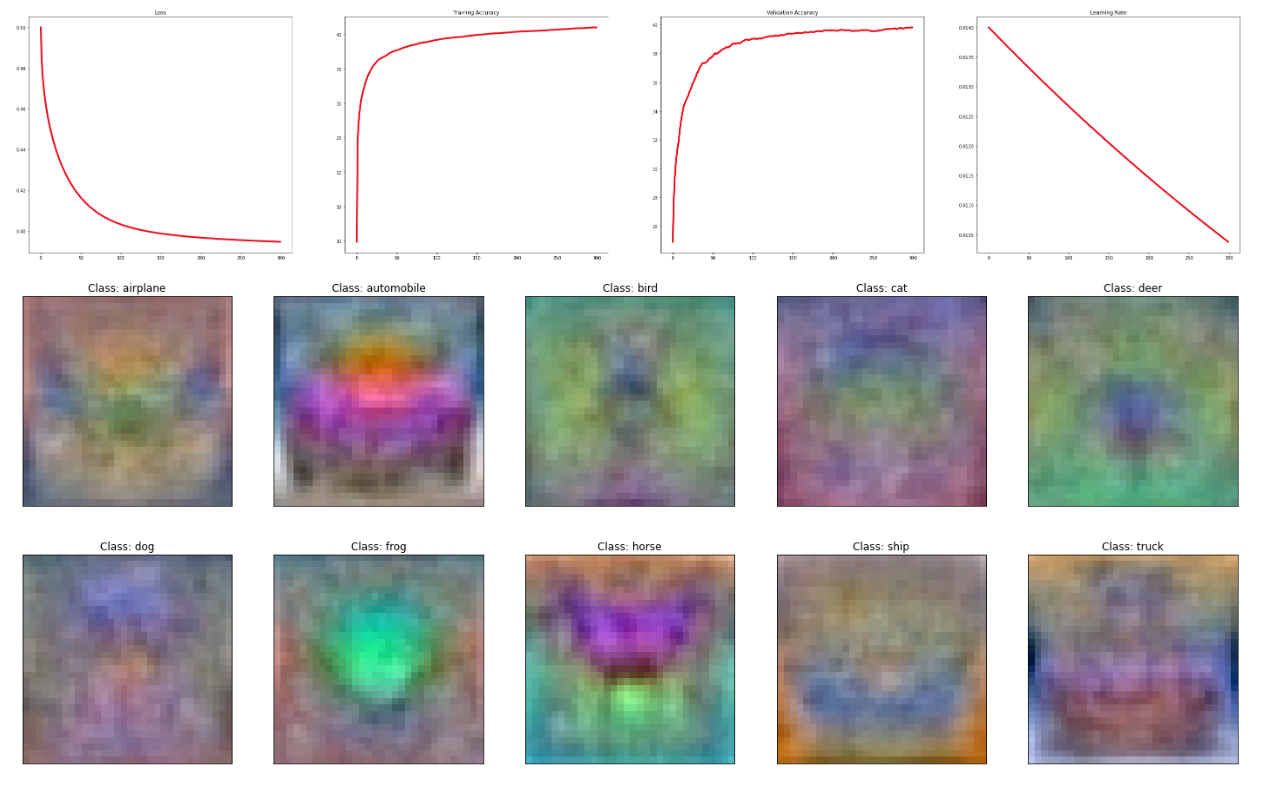
\includegraphics[width=0.9\linewidth]{1_2.PNG}
  \caption{Sample Caption: Learning and loss curves}
  \label{fig:sub1}
\end{subfigure}%
\begin{subfigure}{0.5\textwidth}
  \centering
  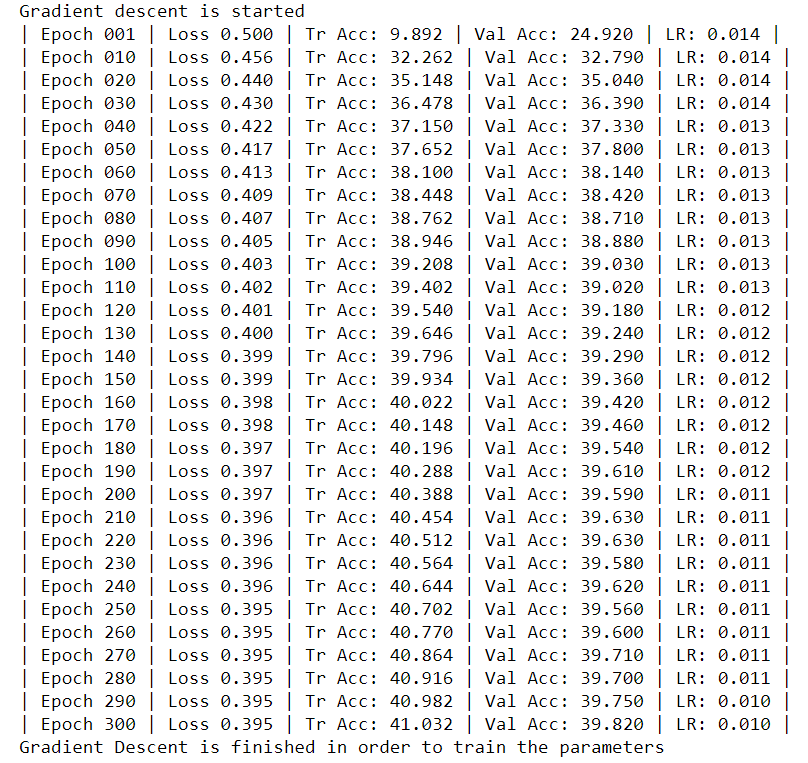
\includegraphics[width=0.7\linewidth]{1_1.PNG}
  \caption{Sample Caption: Numerical values of the losses and accuracies}
  \label{fig:sub2}
\end{subfigure}
\caption{Sample caption: Acquired results through the implemented linear classifier}
\label{fig:test}
\end{figure}
\end{enumerate}

\paragraph*{Problem 2}
Sample Question: Code a two-layer fully connected network with $H = 200$ hidden nodes. Choose the sigmoid function as the activation function for the hidden nodes. The output layer has no activation function.
\begin{enumerate}[label=(\alph*)]
\item Sample Sub-question: Implement gradient descent and run for 300 epochs.
\newline Sample Answer: \textbf{Lorem Ipsum} is simply dummy text of the printing and typesetting industry. Lorem Ipsum has been the industry's standard dummy text ever since the 1500s, when an unknown printer took a galley of type and scrambled it to make a type specimen book. It has survived not only five centuries, but also the leap into electronic typesetting, remaining essentially unchanged.

\begin{equation}
    \frac{dl}{dw2} = \frac{dl}{dpredict} X \frac{dpredict}{dw2}
\end{equation}

\begin{equation}
    \frac{dl}{dw1} = (\frac{dl}{dpredict}X\frac{dpredict}{dh})X(\frac{dh}{dw1x}X\frac{dw1x}{dw1})
\end{equation}

\item Sample Sub-question: Report the (initial) learning rate, training and testing loss and accuracies.
\newline Sample Answer: Lorem Ipsum is simply dummy text of the printing and typesetting industry. Lorem Ipsum has been the industry's standard dummy text ever since the 1500s, when an unknown printer took a galley of type and scrambled it to make a type specimen book. It has survived not only five centuries, but also the leap into electronic typesetting, remaining essentially unchanged.
\end{enumerate}


\paragraph*{Problem 3}
Sample Question: Modify the code in item 2 to carry out stochastic gradient descent with a batch size of 500 (Report training and testing loss and accuracies and Compare results with item 2).

\newline Sample Answer: Lorem Ipsum is simply dummy text of the printing and typesetting industry. Lorem Ipsum has been the industry's standard dummy text ever since the 1500s, when an unknown printer took a galley of type and scrambled it to make a type specimen book. It has survived not only five centuries, but also the leap into electronic typesetting, remaining essentially unchanged.


\begin{figure}[H]
    \centering
    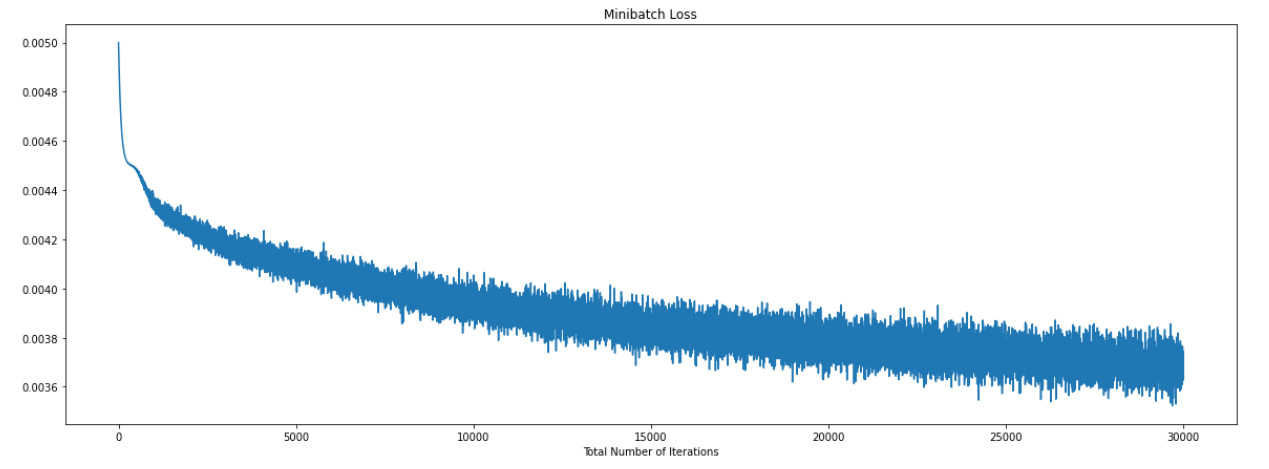
\includegraphics[width=0.6\textwidth]{3_2.PNG}
    \caption{Sample Caption: Mini-batch loss vs total number of iterations }
    \label{fig: PaleBlueDot}    
\end{figure}

Lorem Ipsum is simply dummy text of the printing and typesetting industry. Lorem Ipsum has been the industry's standard dummy text ever since the 1500s, when an unknown printer took a galley of type and scrambled it to make a type specimen book. It has survived not only five centuries, but also the leap into electronic typesetting, remaining essentially unchanged.

\paragraph*{Problem 4}
Sample Question: Construct a CNN using \textit{Keras.models.Sequential} (with the following configuration: C32, C64, C64, F64, F10. All three convolutions layers are 3x3. Max pooling (2x2) follows each convolution layer. Use SDG (with momentum) with a batch size of 50 and \textit{CategoricalCrossentropy} as the loss (Include how many learnable parameters are there in this network?, report the parameters such as the learning rate and momentum and Report training and testing loss and accuracies)

Sample Answer: Lorem Ipsum is simply dummy text of the printing and typesetting industry. Lorem Ipsum has been the industry's standard dummy text ever since the 1500s, when an unknown printer took a galley of type and scrambled it to make a type specimen book. It has survived not only five centuries, but also the leap into electronic typesetting, remaining essentially unchanged. 

\begin{center}
$loss=-\sum_{i=1}^{outputSize} y_iX\log{\hat{y_i}}$. 
\end{center}

\bibliography{references}

\end{document}
%Compiled by Nuwan Bandara, ENTC, University of Moratuwa, Sri Lanka

